\documentclass[final, letterpaper, square, comma, numbers, sort&compress]{elsarticle}
\usepackage[utf8]{inputenc}
\usepackage[
    % margin=1in
    top=1in,
    bottom=0.5in,
    left=1in,
    right=1in,
    footskip=0.25in, % FIXME: temp fix
    % showframe % Uncomment to show frames around the margins for debugging purposes
]{geometry}

\usepackage{hyperref}
\hypersetup{
	% colorlinks=true, % Whether to color the text of links
	% urlcolor=black, % Color for \url and \href links
	% linkcolor=black, % Color for \nameref links
	% citecolor=black, % Color of reference citations
        hidelinks,
        pdfauthor={R. Ranjan; J. Wilson; M. Barisik; V. Ramanuj; R. Sankaran;},
        pdftitle={Effects of Operating Conditions on the Gas-Phase Decomposition of MTS/H2 during Chemical Vapor Infiltration of SiC} % these lines are nessesary to avoid hyperref throwing errors from pulling the newline in the given frontmatter title section
}

\usepackage{graphicx}
\graphicspath{{figures/}}
\usepackage{amssymb}
% \usepackage{gensymb} % not needed

%% The amsthm package provides extended theorem environments
%% \usepackage{amsthm}

\journal{Energy Policy} % FIXME

\begin{document}

\begin{frontmatter}

%% Title, authors and addresses
\title{Effects of Operating Conditions on the Gas-Phase Decomposition of \\ MTS/H$_2$ during Chemical Vapor Infiltration of SiC}

\author[1]{R.~Ranjan\corref{cor1}}
\ead{reetesh-ranjan@utc.edu}
\author[1]{J.~Wilson}
\author[1]{M.~Barisik}
\author[2]{V.~Ramanuj}
\author[2]{R.~Sankaran}
\cortext[cor1]{Corresponding author}

\address[1]{Department of Mechanical Engineering, The University of Tennessee Chattanooga \\
615 McCallie Avenue, Chattanooga, TN 37403, USA}
\address[2]{Computational Sciences and Engineering Division, Oak Ridge National Laboratory \\
1 Bethel Valley Rd., Oak Ridge, TN 37831, USA}

\begin{abstract}
The quality of the silicon carbide (SiC) matrix composite, which has excellent thermo-mechanical properties, fabricated by the well-established chemical vapor infiltration (CVI) process, depends upon the gas-phase decomposition of the employed precursor and the subsequent heterogeneous reactions at the deposition surface. The decomposition process is primarily affected by the operating parameters such as temperature, pressure, gradient of pressure and temperature, and the composition of the incoming gas-phase reactants. In this study, we perform plug flow reactor (PFR) analysis to examine the effects of operating parameters on the decomposition of the mixture of methyltrichlorosilane (MTS) and hydrogen ($\rm H_2$), a widely used precursor for the manufacturing of SiC matrix composite using the CVI process. The PFR analysis is performed using three chemical mechanisms of increasing degree of complexity, which include globally reduced (1 step and 5 species), moderately complex (30 steps and 20 species), and detailed (103 steps and 42 species) mechanisms. First, we discuss the reduction strategy to obtain the moderately complex mechanism from the detailed one and assess the performance of the three mechanisms by comparing PFR results at atmospheric pressure with reference experimental and numerical results. Afterward, the PFR analysis is performed using these mechanisms at conditions relevant to CVI. These include a range of temperature (1100 K to 1600 K), pressure (5 Torr to 100 Torr), temperature gradient (-190 K/m to -19 K/m), and pressure gradient (-7.7 Torr/m to -0.97 Torr/m). The analysis of the results pertaining to the decomposition of MTS and production of several intermediate reactive species shows that the decomposition of MTS is more sensitive to temperature and its gradient than pressure or pressure gradient. The effects of the ratio of MTS and H2 in the incoming mixture (0.05 to 0.2) are examined by considering isothermal and temperature-gradient conditions. The results show enhanced decomposition of MTS in the case with the presence of a temperature gradient for the same mixture composition, and a nonlinear dependence of the decomposition of MTS and production of intermediates and byproducts on the incoming mixture composition. The present study also showed that the moderately complex chemical kinetics show good agreement with the detailed mechanism, whereas the globally reduced chemical mechanism yielded inaccurate results, thus implying that the moderately complex mechanism can be used while performing detailed three-dimensional modeling of the CVI process.
\end{abstract}

\begin{keyword}
Chemical vapor infiltration \sep silicon carbide \sep methyltrichlorosilane \sep plug flow reactor \sep chemical mechanisms
\end{keyword}

\end{frontmatter}

\let\thefootnote\relax\footnote{Notice: This manuscript has been authored by UT-Battelle, LLC, under contract DEAC05-00OR22725 with the US Depart-ment of Energy (DOE). The US government retains and the publisher, by accepting the article for publication, acknowledges that the US government retains a nonexclusive, paid-up, irrevocable, worldwide license to publish or reproduce the published form of this manuscript, or allow others to do so, for US government purposes. DOE will provide public access to these results of federally sponsored research in accordance with the DOE Public Access Plan (\bf \href{http://energy.gov/downloads/doe-public-access-plan}{http://energy.gov/downloads/doe-public-access-plan}).}

\section{Introduction}
\label{S:1}

Materials that can withstand high-temperature environments are required in many engineering applica- tions such as nuclear reactors, automotive, spacecraft, aircraft components, furnace linings, power electronics,
and cutting and grinding tools. Such materials include metals and alloys (titanium alloys, tungsten, molyb- denum), ceramics (alumina, silicon carbide (SiC), graphite), and composites (ceramic matrix composites, carbon-carbon composites)~\cite{Meetham1991,Tressler1999,Belmonte2006,Fahrenholtz2014,BarCohen2014}. SiC is one such material, which has excellent properties such as high strength, high thermal conductivity, low thermal expansion, chemical inertness, and good thermal shock strength~\cite{Levinshtein2001,Hironaka2002,Snead2007,Presser2008}. However, it also tends to have a low toughness~\cite{Padture1994,Mulla1994,Cao1995}, which has motivated interest in high purity and high quality SiC fiber-reinforced matrix composites~\cite{Naslain1995,Prewo1989,Besmann1991,Wang1996,Prouhet1994,Zhu1999,Liu2023}. In such composites, a SiC matrix is deposited within a fiber preform composed of high-purity, near-stoichiometric SiC fiber. Such an approach leads to a better fracture toughness property while still having a similar performance under high thermal- loading conditions. The deposition of the SiC matrix composites depends upon the operating conditions, which affect the gas-phase decomposition and the subsequent heterogeneous surface reactions on the fiber preform. The present study examines the effects of operating conditions on the gas-phase decomposition of the precursor and the production of intermediate reactive species during SiC matrix deposition.


SiC matrix composites can be fabricated using approaches such as melt infiltration~\cite{Xu1999,DiCarlo2005}, polymer infiltration and pyrolysis~\cite{Sirieix1990, Kohyama2000}, and chemical vapor infiltration (CVI)~\cite{Sayano1999,Lamon2005,Deck2013}. Past studies have shown that CVI is a reliable approach to obtain a very high-purity SiC matrix composite~\cite{Lamon2005,Katoh2014}. During the CVI process, a SiC precursor is introduced into a chamber in the gas phase, which diffuses into the fiber preform and chemically reacts, forming a SiC matrix within the sample. There are two major challenges associated with the CVI process, which affect the overall quality of the resultant matrix composite. The first challenge is associated with the processing time. While CVI produces a very high-purity matrix, as the deposition process is dependent on the diffusion of reactants into the fiber preform, ideally, a slow reaction rate is desirable to ensure uniform transport of reactants throughout the preform. However, with a slower reaction rate, the processing time gets longer, which can affect the quality of the resulting composite. For example, high porosity can be observed, and filling of inter-tow sharp and large pores can be a challenge while keeping the processing times low~\cite{Liu2021}. Therefore, modifications have been considered to the conventional CVI process~\cite{Lamon2005,Probst1999}. These include thermal-gradient CVI~\cite{Stinton1986}, pressure-gradient CVI (forced flow CVI)~\cite{Deck2013}, pressure-pulsed CVI~\cite{Naslain2001}, and whisker-growing assisted CVI~\cite{Oh2001}. The second challenge is related to the dependence of the quality of the SiC deposition on the gas-phase decomposition of the precursor that is used during the process. Note that the precursor decomposition and production of the reactive intermediates directly affect the heterogeneous surface reactions and can also affect the overall processing time. This particular challenge can be addressed by studying the effects of operating conditions on the decomposition of the precursor used for the CVI of SiC matrix composite, which is the major focus of this study.

Some of the commonly used precursors for the fabrication of SiC through the CVI process include methyltrichlorosilane ($\rm CH_3SiCl_3$), hereafter referred to as MTS, silane ($\rm SiH_4$) along with hydrocarbons such as methane ($\rm CH_4$), dichloromethylsilane ($\rm CH_3SiHCl_2$), and hexamethyldisilane ($\rm (CH_3)_6Si_2$)~\cite{Noda1992,Naslain2006,Lazzeri2012}. Out of these, MTS is widely used as it yields a perfect stoichiometry (1:1 Si:C), leading to high-purity SiC with minimal free carbon or silicon~\cite{Lamon2005}. In addition, its decomposition characteristics can be controlled by varying operating temperature (800 to 1000 $^o$C) and pressure (5 to 100 Torr) conditions, and the ratio of MTS to hydrogen ($\rm H_2$) in the incoming mixture. Note that MTS is used as a precursor along with $\rm H_2$ as the carrier gas, which in turn can suppress free carbon formation and reduce volatile intermediates such as $\rm SiCl_4$~\cite{Lazzeri2012}. Therefore, in this study, we study the decomposition characteristics of MTS, which can lead to the production of several intermediate reactive species such as $\rm CH_4$, HCl, $\rm SiCl_4$, $\rm SiHCl_3$, etc., that in turn affect the deposition process at the preform surface where heterogeneous reactions occur.

The computational study of CVI of SiC matrix composite can be carried out using techniques with varying levels of fidelity and computational cost, which include, computational fluid dynamics (CFD)~\cite{Streitwieser2006,Ramadan2018,Cha2022,Ramanuj2022}, direct simulation Monte Carlo (DSMC)~\cite{Deck2013,Deck2012}, or plug-flow reactor (PFR)~\cite{Dang2022}. For example, while CFD can simulate large-scale fabrication systems and account for transport and diffusion processes, it faces challenges in accurate modeling of the matrix infiltration process, where the transport of the reactants occurs through the fiber preform, leading to Knudsen numbers much larger than unity. To this end, the DSMC technique can be employed, although it is computationally expensive for the simulation of large-scale fabrication systems. While using either of these techniques, accurate modeling of chemical kinetics is pivotal to the accuracy of the prediction of the gas-phase decomposition and subsequent deposition through the heterogeneous surface reactions on the fiber preform. However, due to computational complexities associated with detailed chemical kinetics, often simplified chemical mechanisms are employed while using CFD and DSMC techniques~\cite{Deck2012,Mollick2017,Ogawa2023}, which tend to yield inaccurate results. Therefore, there is a need to have reliable yet affordable chemical mechanisms that can accurately predict the gas-phase decomposition and subsequent heterogeneous reactions during CVI of SiC. In this study, we employ a plug-flow reactor (PFR) as the computational technique, which can efficiently account for detailed chemical kinetics~\cite{Papasouliotis1994,Roman1995,Bammidipati1996,Norinaga2008} to study the decomposition of MTS under different operating conditions. In a PFR, a steady flow field within an axial duct is modeled, where the flow in the transverse direction is considered to be completely homogeneous.

The key objective of this study is to first establish a PFR setup, and then to use the setup to examine the effects of operating conditions on the gas-phase decomposition of MTS and production of intermediate reactive species such as $\rm CH_4$, HCl, $\rm SiHCl_3$, $\rm SiCl_2$, and $\rm SiCl_4$ under CVI-relevant conditions. Past studies using PFR have primarily focused on the development and assessment of chemical kinetics, and therefore, the present study will complement the findings of such studies. Along with the detailed kinetics, we also assess the performance of two other chemical mechanisms, which can be potentially used with CFD and DSMC simulations. The three chemical mechanisms include detailed (103 steps and 43 species)~\cite{Ge2007A,Ge2007B,Ge2010}, moderately complex reduced (30 steps and 20 species), and globally reduced (1 step and 5 species)~\cite{Mousavipour2004} mechanisms. The moderately complex mechanism is obtained using a reduction technique (discussed later) in the present study. To examine the decomposition of MTS in the presence of $\rm H_2$, we consider different CVI reactor conditions. Apart from considering a range of operating temperatures (1100 K to 1600 K) and pressures (5 Torr to 100 Torr), we also examine the effects of a range of temperature gradients (-190 K/m to -19 K/m), and pressure gradients (-7.7 Torr/m to -0.97 Torr/m). Past studies have also shown that the decomposition of MTS is affected by the composition, i.e., molar ratio of MTS/$\rm H_2$ ($\beta$)~\cite{Peng2021}. Therefore, the effects of variation in $\beta$ (0.05 to 0.2) are also examined after identifying optimal operating temperature and pressure conditions. 

This article is arranged as follows. The details for the computational setup and the employed numerical methodology are presented in Section 2. In Section 3, an assessment of the PFR-based computational strategy is performed by comparing the results with reference data from the literature. The results of this study are discussed in Section 4. Finally, the key outcomes of this study are summarized in Section 5.


\begin{figure}[t]
\centering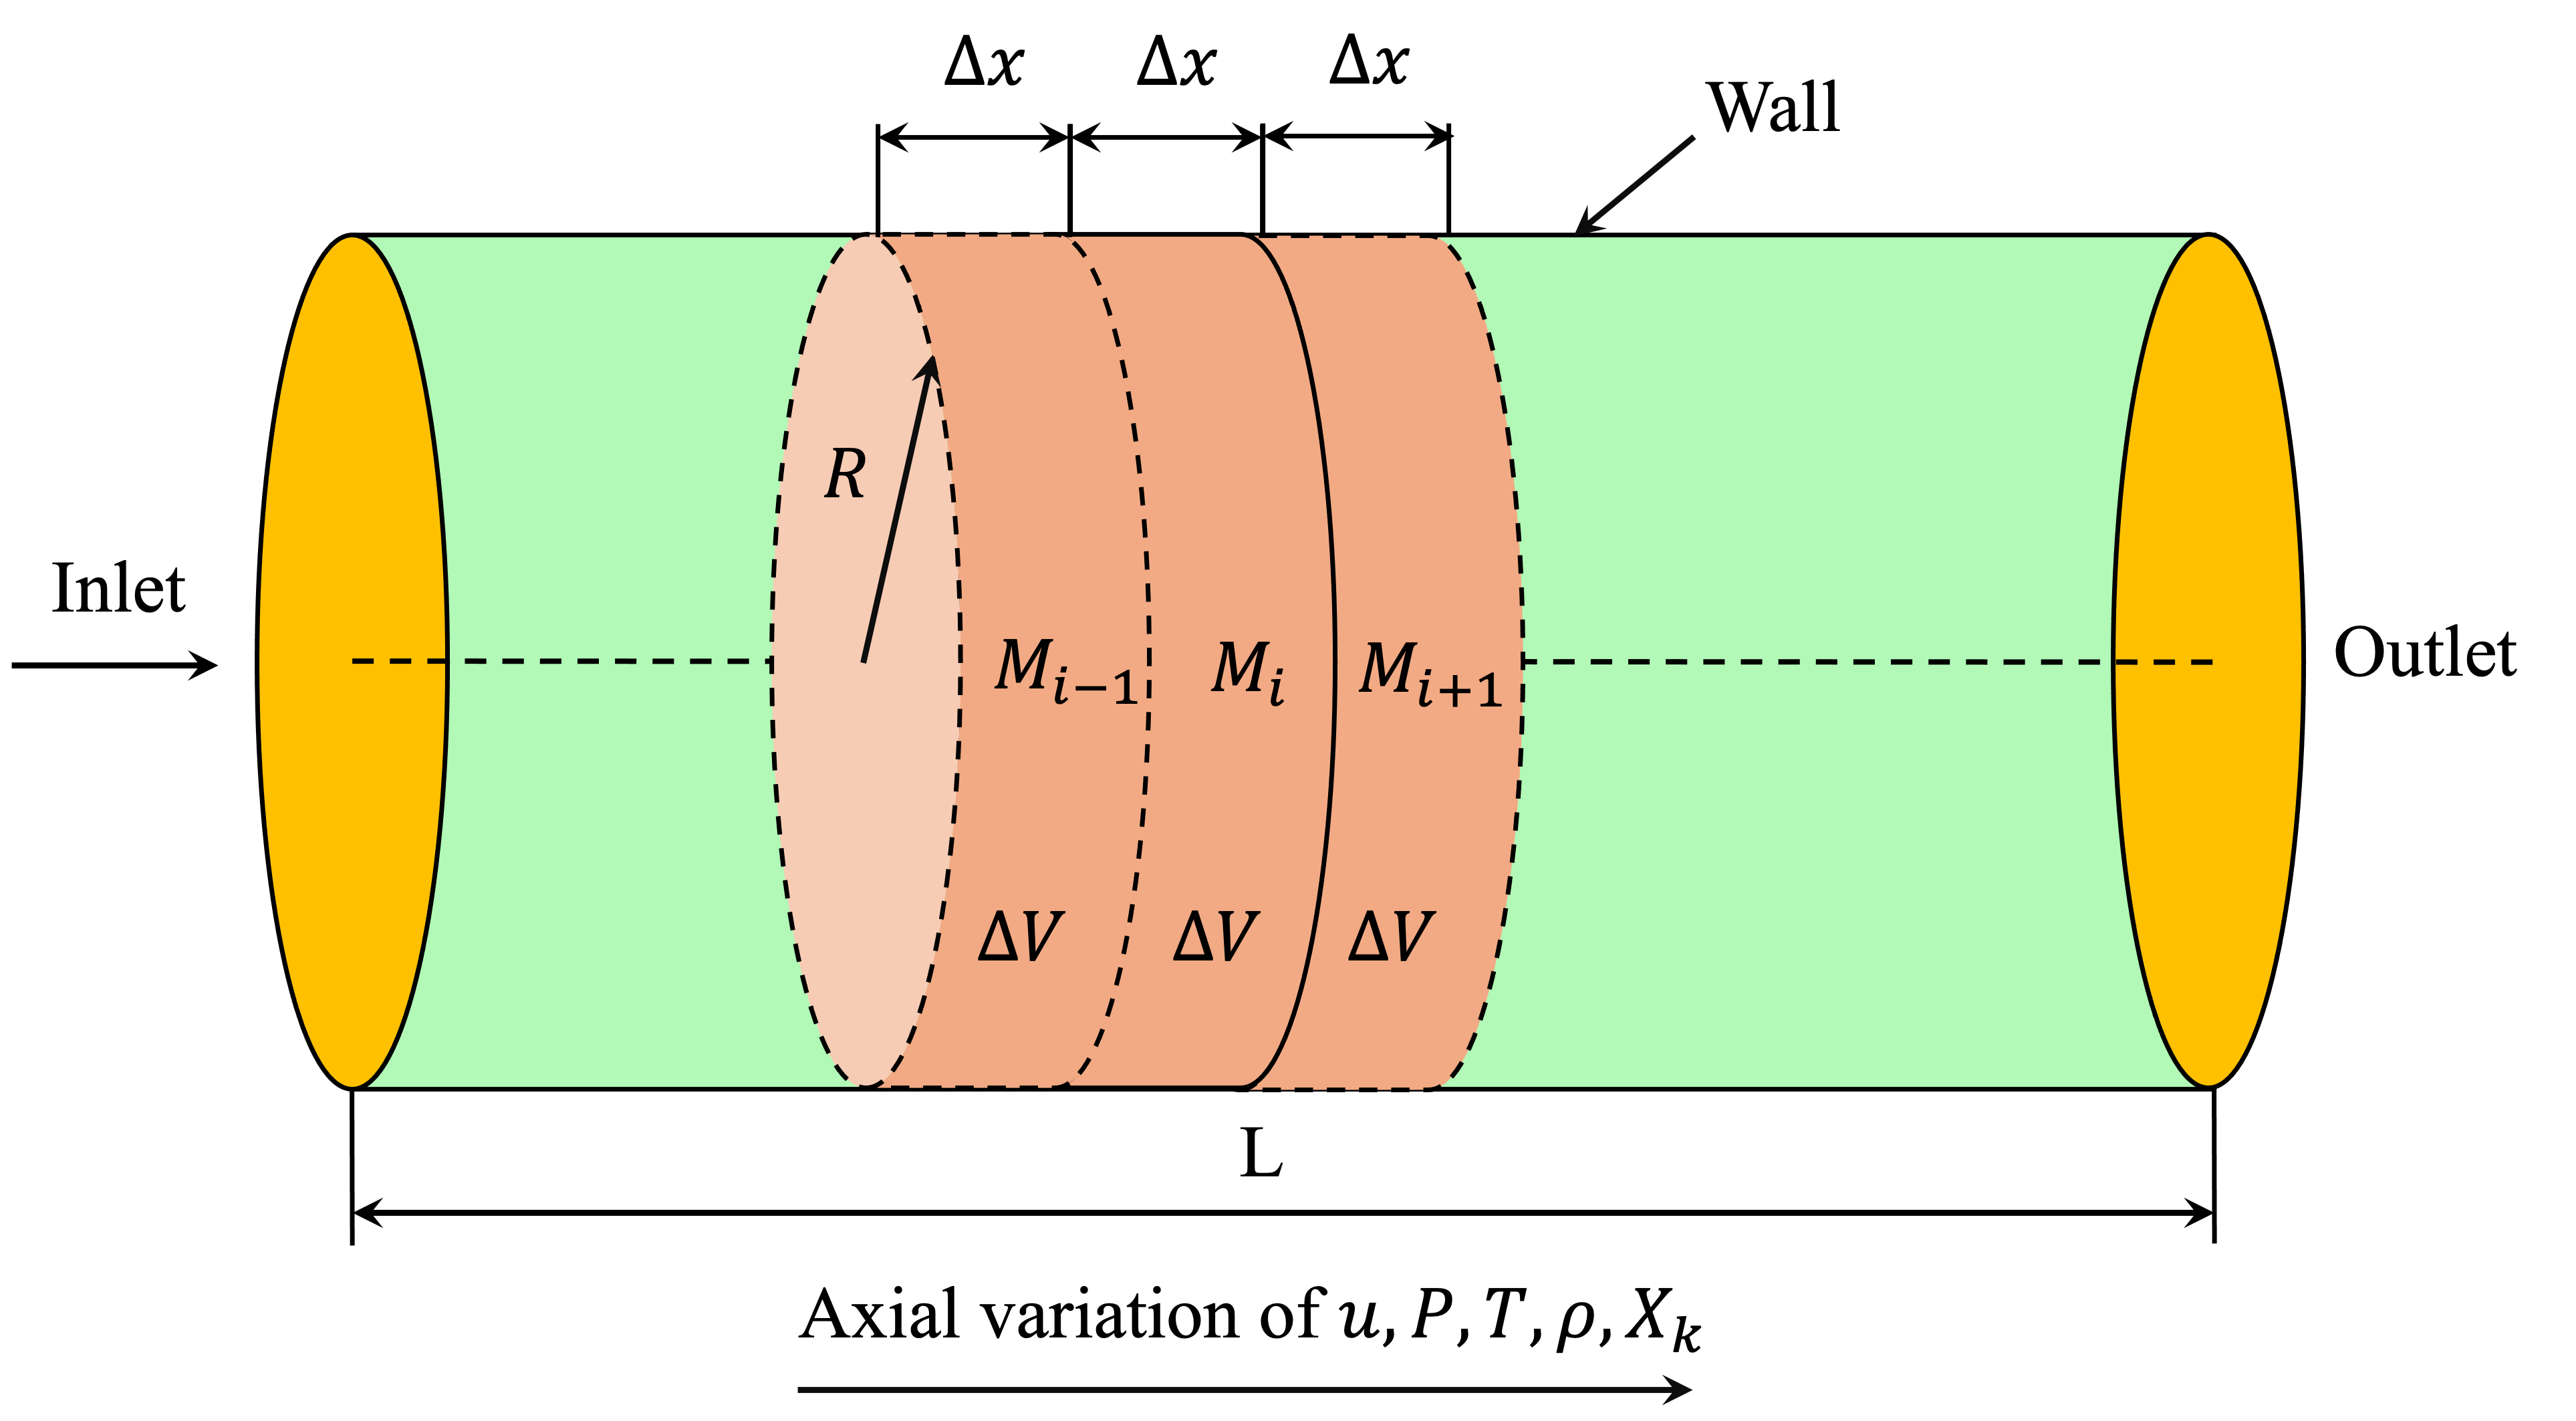
\includegraphics[width=0.6\textwidth]{PFR-schematic.png}
\caption{Schematic of a plug flow reactor-based representation of the hot-wall CVI reactor configuration. Here, $M_i$ denotes the $i^{th}$ plug along the axial ($x$) direction, and $\Delta x$, $\Delta V$, and $R$ denote the axial length, volume, and radius of the plug, respectively.}
\label{PFR-schematic}
\end{figure}

\section*{Acknowledgements}
This work was supported by the U.S. Department of Energy, Office of Science, Office of Basic Energy Sciences (BES), Gas Phase Chemical Physics (GPCP) through Grant \#DE-SC0024510.

%% References with bibTeX database:
\bibliographystyle{elsarticle-num}
\bibliography{cvi-bib}

\end{document}
